\subsection{Ripeness Detection}
\subsubsection{Data}
The data for this model was a subset of the Fruits360 data set~\cite{Fruit360}.
Unable to find any suitable data sets showing a single apple species at different stages of ripeness, we settled for using two ripe, similar looking apple species.
In the Fruits360 data set~\cite{Fruit360}, we used crimson snow apples to represent ripe apples, and the data set's ``red 2'' apples to represent unripe apples. We  chose to use these since the two types had a very similar shape in their images, making the biggest variation between them the color which is what our model focuses on.

\subsubsection{Model}
The ripeness of an apple is determined by an SVM classifier model based on the HSV values of the apple image because it has been shown to be capable of having a high accuracy at fruit ripeness detection~\cite{HSVRipeness}.
The model takes an input feature vector based on the histogram calculation of an HSV image measuring $(100$pixels$\times100$pixels), Using OpenCV and python.
Within OpenCV, hue is a number from 0 to 179, inclusive, and saturation and value are both numbers from 0 to 255, inclusive.
These calculation values then get flattened down into a 1-dimensional feature vector storing 689 numbers. 
This feature vector is used as input for our SVM classifier. Below is an example of a ripe apple, and its HSV histogram calculation values. The $y$ value of each point of each line is the amount of times that value of H, S, or V appears in the image.\\
\begin{figure}[!htb]
    \fontsize{7}{5}\selectfont
    \centering
    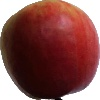
\includegraphics[scale=0.7]
    {figures/Ripe Apple Example.jpg}
    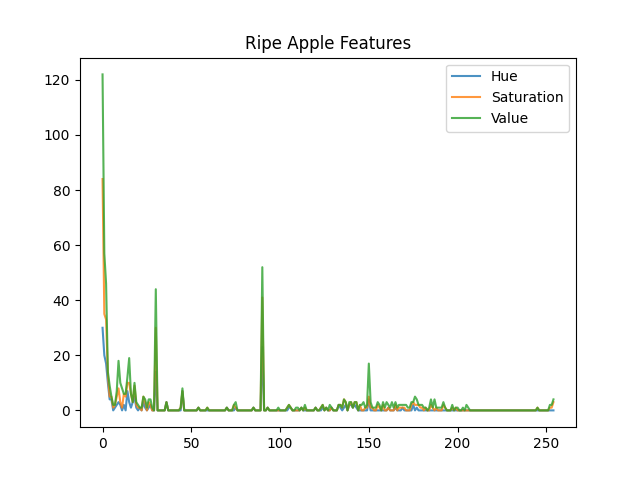
\includegraphics[scale=.5]
    {figures/ripeness_features.png}
    \label{Ripe Apple Example}
    \caption{
        A ripe apple, and its associated HSV histogram calculations from the image preprocessing.
    }
\end{figure}

\subsubsection{Improvements}
Because we were unable to find data focused more specifically on detecting ripeness, 
one good way to improve the performance of our project would be to gather picture of both ripe and unripe variants of whatever apple species the drone would be targeting. 
To make this model production ready, it would likely require a new ripeness model to be trained for each species of apple targeted.
Also, the model is currently trained on images of apples over a white background, for a production environment this would likely be much less effective.
